\section{Analysis of the dataset}

\begin{frame}{Analysis of the dataset}
	\textbf{Video data:}
	\begin{itemize}
		\item<+-> frame size of $(640,480,3)$ pixels
		\item<+-> cut off last 60 pixels, to remove black frame inside the car
		\item<+-> sample down the frame to half its size, to reduce computation time
	\end{itemize}
	
	\begin{columns}[t]
		\begin{column}{.45\textwidth}
			\begin{center}
				\only<1->{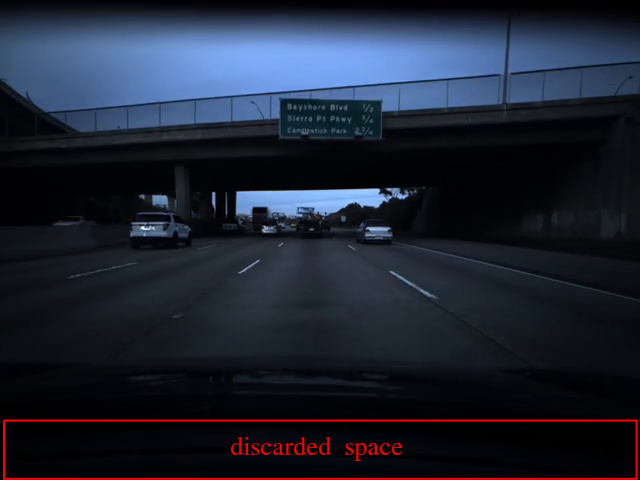
\includegraphics[width=\linewidth]{./imgs/frame2_evaluated.png}}
				\small{Original frame}
			\end{center}
		\end{column}
		\begin{column}{.45\textwidth}
			\begin{center}
				\only<3->{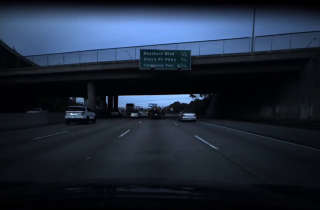
\includegraphics[width=\linewidth]{./imgs/frame2_cut_sampled.png}}
				\small{Cut off the last 60 pixels, downsampled}
			\end{center}
		\end{column}
	\end{columns}
\end{frame}

\begin{frame}{Analysis of the dataset}
	\begin{columns}[c]
		\begin{column}{.55\textwidth}
			\textbf{Splitting of the dataset}
			\begin{itemize}
				\item<+-> Initial splitting: hard cut off after $80\%$ of the frames
				\item<+-> Situational splitting: divide dataset into blocks of different driving scenarios,
				splitting with $80\%$ test and $20\%$ validation data on each
%				\setbeamertemplate{itemize items}[circle]
%				\begin{itemize}
%					\item divide dataset into blocks of different categories
%					\item splitting with $80\%$ test and $20\%$ validation data on each
%				\end{itemize}
			\end{itemize}
			\pause
			\textbf{Evaluation:}
			\begin{itemize}
				\item<+-> variance $\sqrt{\mathcal{L}} \gtrsim 16$: no fitting
				\item<+-> $10 \lesssim \sqrt{\mathcal{L}} \lesssim 16$: average velocity fitted
				\item<+-> $5 \lesssim \sqrt{\mathcal{L}} \lesssim 10$: qualitative detection
				\item<+-> $1 \lesssim \sqrt{\mathcal{L}} \lesssim 5$: quantitative detection
				\item<+-> $\sqrt{\mathcal{L}} \lesssim 1$: perfect detection
			\end{itemize}
		\end{column}
		\begin{column}{.45\textwidth}
			\begin{center}
				\only<1->{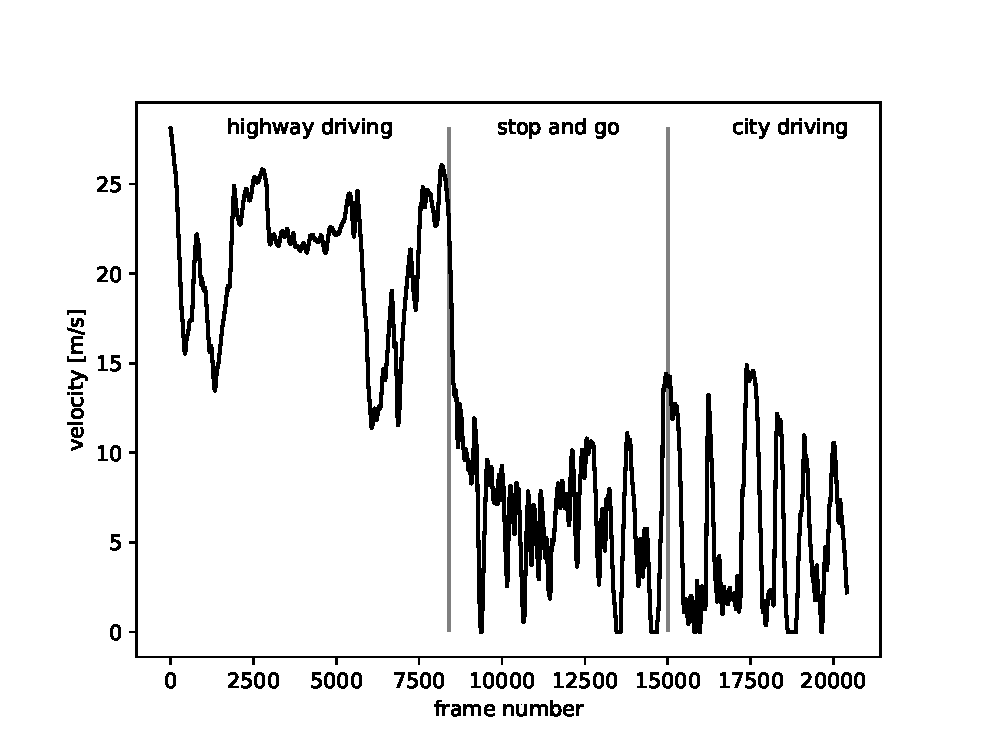
\includegraphics[width=0.85\textwidth, height=0.34\textheight]{./imgs/plot_speed_time_new_splitting.eps}
				{\footnotesize driving situations in v-t-plot}}
				\only<5->{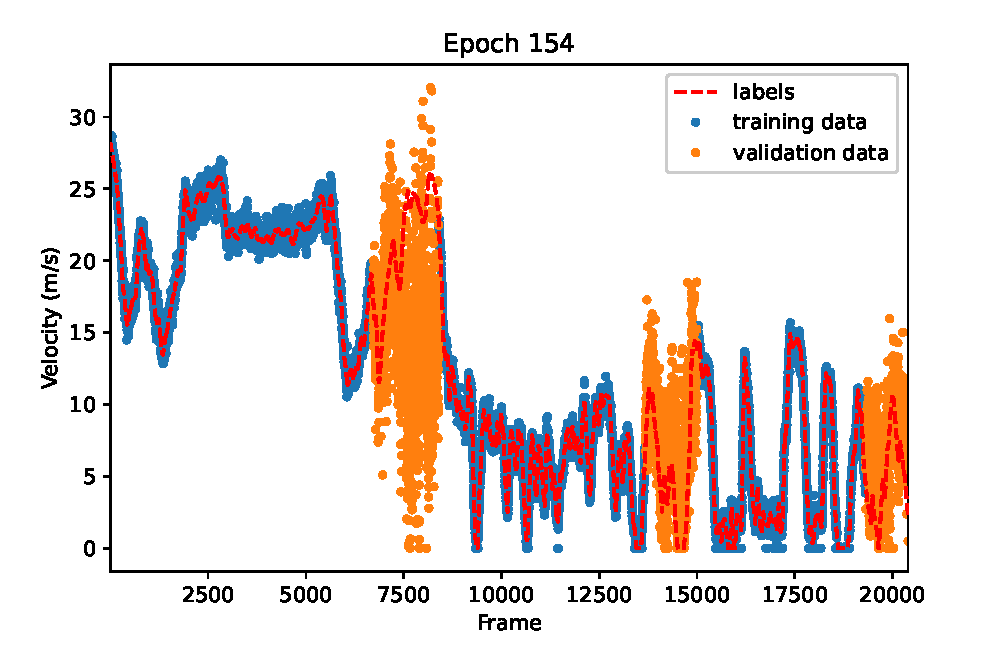
\includegraphics[width=0.85\textwidth]{./imgs/example_performance.eps}
				{\footnotesize example performance on training set \\ training: $\sqrt{\mathcal{L}}=0.4$, test: $\sqrt{\mathcal{L}}=6.3$}}
			\end{center}
		\end{column}
	\end{columns}
\end{frame}